\chapter{Isabelle/HOL}\label{chapter:isabelle}

Isabelle is a theorem prover implemented in Standard ML, which supports multiple logical systems. We use Isabelle/HOL (Higher-Order Logic), the most used logical system, and the Isabelle/Isar framework, which provides a structured proof language (Isar-ref). For more detailed descriptions of Isabelle, we refer to [Isar-ref] and [prog-prove].

\section{Imperative/HOL}

Imperative/HOL is a framework, built on Isabelle/HOL, for reasoning about imperative programs and data structures. It works with a polymorphic heap model and a "Haskell-like" state-exception monad [link]. The monadic setup allows straight-forward implementations of programs in do-notation [link] using both imperative and functional language constructs. It also supports efficient code generation for various target languages like SML, OCaml, Haskell, and Scala. Additionally, already existing proof automation tools of Isabelle/HOL are easily reusable (Bulwahn 2008, 134).
The heap consists of two mappings, which describe references to values and arrays, and a counter which bounds the currently used address space (Bulwahn 2008, 140). This heap is the state of the of the state-exception monad, in which imperative programs can be represented (Bulwahn 2008, 140f). Like that, an imperative program with the return type $\alpha$ is encoded as a value of type $\alpha$ $Heap$ (Bulwahn 2008, 141).

\begin{figure}[htpb]
    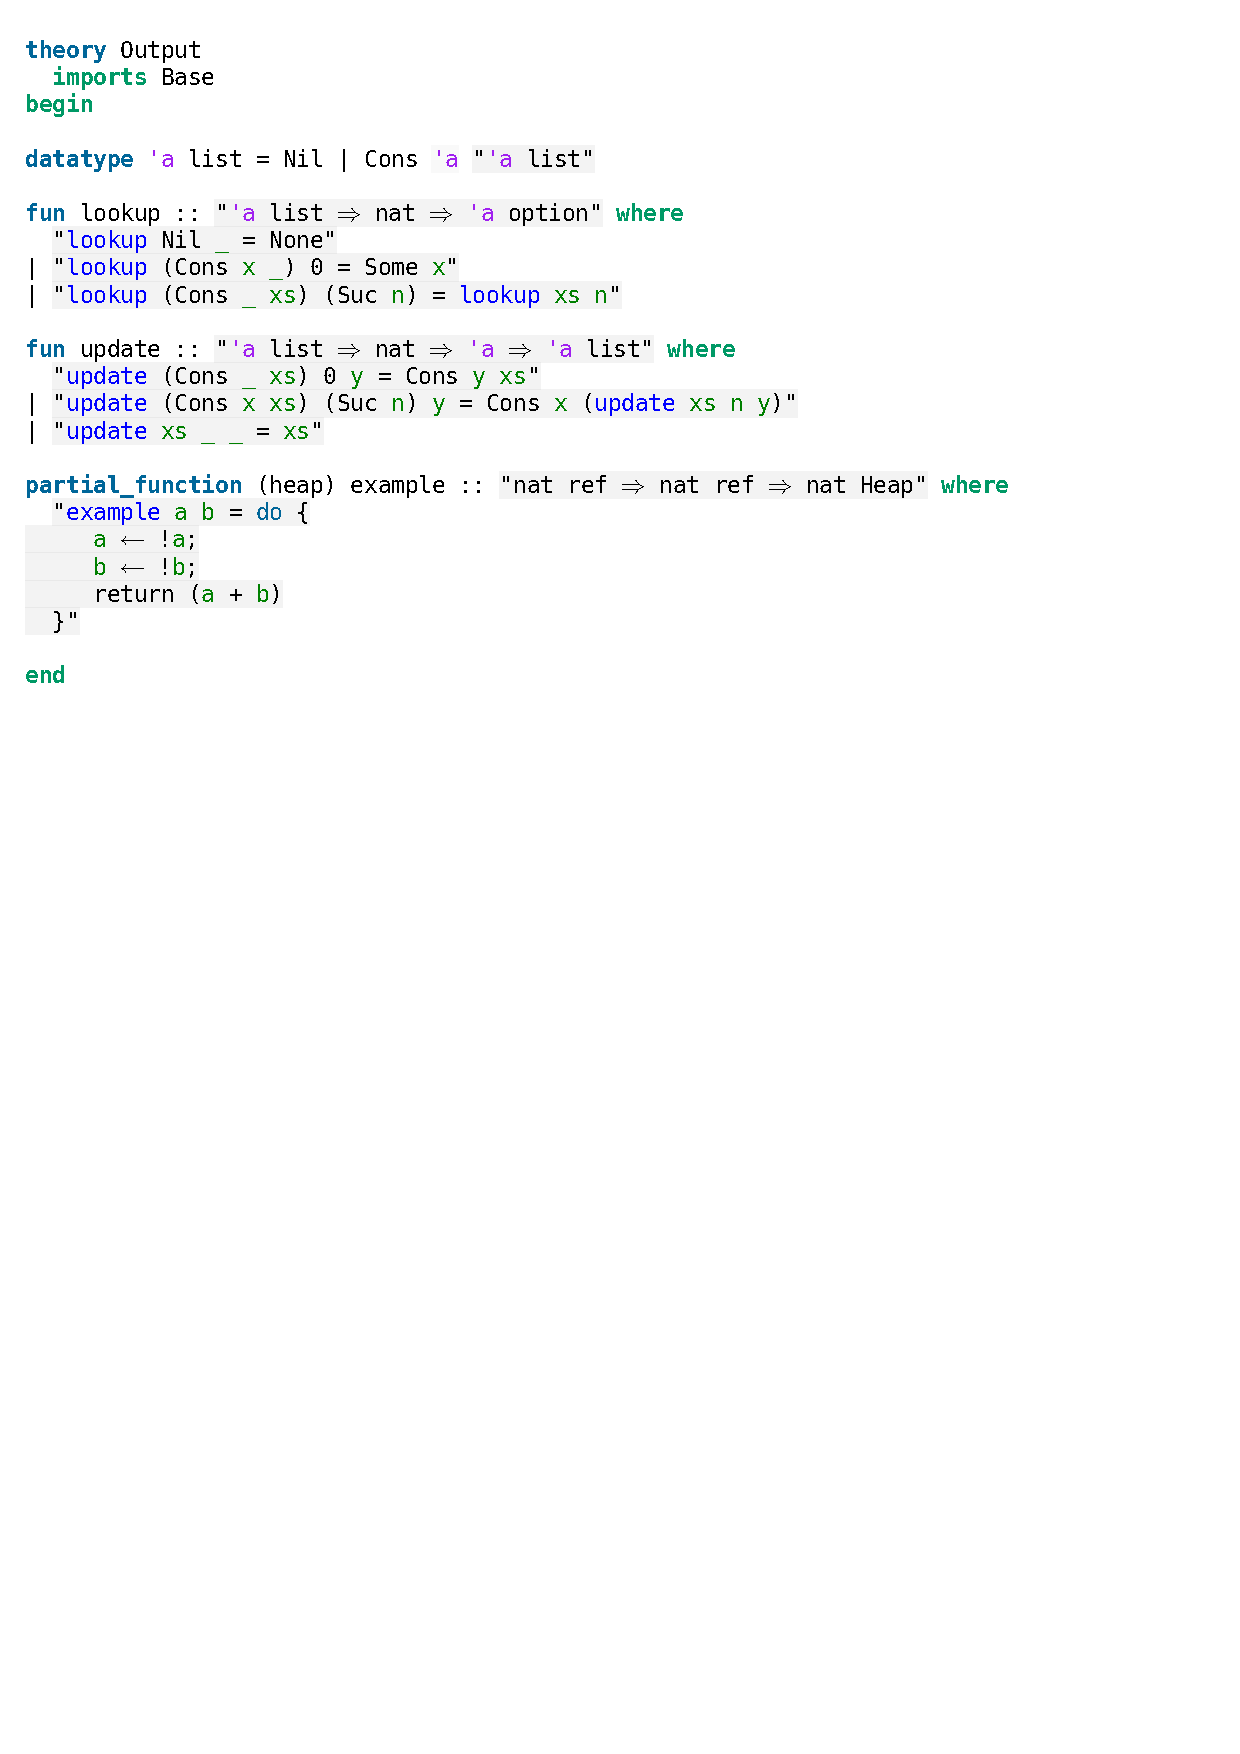
\includegraphics[trim={0 18,9cm 0 8cm}, clip, width=1.00\textwidth]{figures/Theory_Intro.pdf}
    \caption[Imperative/HOL Example]{An example of an imperative function in Imperative/HOL.}
    \label{fig:example-imperative-HOL}
\end{figure}

\noindent \autoref{fig:example-imperative-HOL} is an example using do-notation for a simple addition of two natural numbers stored on the heap. The program first dereferences the two pointers and then returns their sum. 
Because imperative programs inside the monad are not required to terminate and can raise an exception at any point, we need to use |partial|\_|function|s (isar-ref, 263) which support non-termination contrary to the regular |fun|s or |function|s.

